\subsection{Uplifted}

Uplifted is the general name given to the genetically-engineered animals that have been given basic sentience and humanoid features. The original reason behind this science experiment has long been lost, but many speculate that the Uplifted were supposed to perform the menial labour on planets that cannot support a Bot network. Regardless, the Uplifted are still treated as an inferior species because of their artificial evolution.

All Uplifted have the following traits:
\begin{standardtable}{\linewidth}{sb}
  \textbf{Inferior} & Many see the Uplifted as inferior to other species that have evolved naturally. -2 Charisma when other characters deal with the Uplifted.\\
  \textbf{Primal Weapons} & You still have the claws, teeth, horns or other leftovers from your primitive animal state. These natural weapons do Str+d6 damage.\\
  \textbf{Primitive Intellect} & You must spend 2 points per step to raise your Smarts during character creation\\
  \textbf{Free Edge} & (Wild Card only) Start with one free Novice Edge of their choice.\\
\end{standardtable}

In addition, Uplifted have additional abilities due to their animal ancestry. Choose one of the following:

\begin{standardtable}{\linewidth}{sb}
  \textbf{Bear} & Descended from Bears, you are as big (if not bigger) than most Ghoa. +1 Size, and +1 Toughness\\
  \textbf{Bovine} & Descended from Cows, Bulls, and Buffalo. You start with a d6 in Vigor instead of a d4\\
  \textbf{Canine} & Descended from Wolves and Dogs. +2 to Notice when using smell or hearing\\
  \textbf{Feline} & Descended from Lions, Tigers and Panthers. Low-light vision (ignore penalities for dim and dark lighting), and +2 to Athletics climbing checks\\
  \textbf{Rodent} & Descended from Rats, Racoons, and Rabbits. +4 Pace\\
\end{standardtable}

\columnbreak

Uplifted physically range wildly across the spectrum from humanoid to their base animal form, but all Uplifted have at least a humanoid-style torso that have two arms with opposable thumbs (for manipulating objects). Faces may or may not have a prominent snout, and some uplifted do not have a tail. Almost all Uplifted have the fur coat of their base animal base form, but some choose to partially shave or style it to better fit in humanoid society.

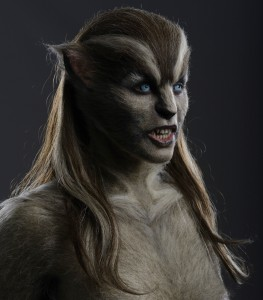
\includegraphics[width=\linewidth]{wolves-movie-still-1-263x300}

Due to their severe genetic alteration and base animal genetics, Uplifted cannot breed with humans or with their animal precedessors. This does not deter kinky humanoids, and many unsavoury places in the Black offer "special" Uplifted services. However the heart wants what it wants, and Uplifted-Human couples are a rare sight in the Black. These couples generally seek out geneticists who are able to splice their DNA into viable offspring.

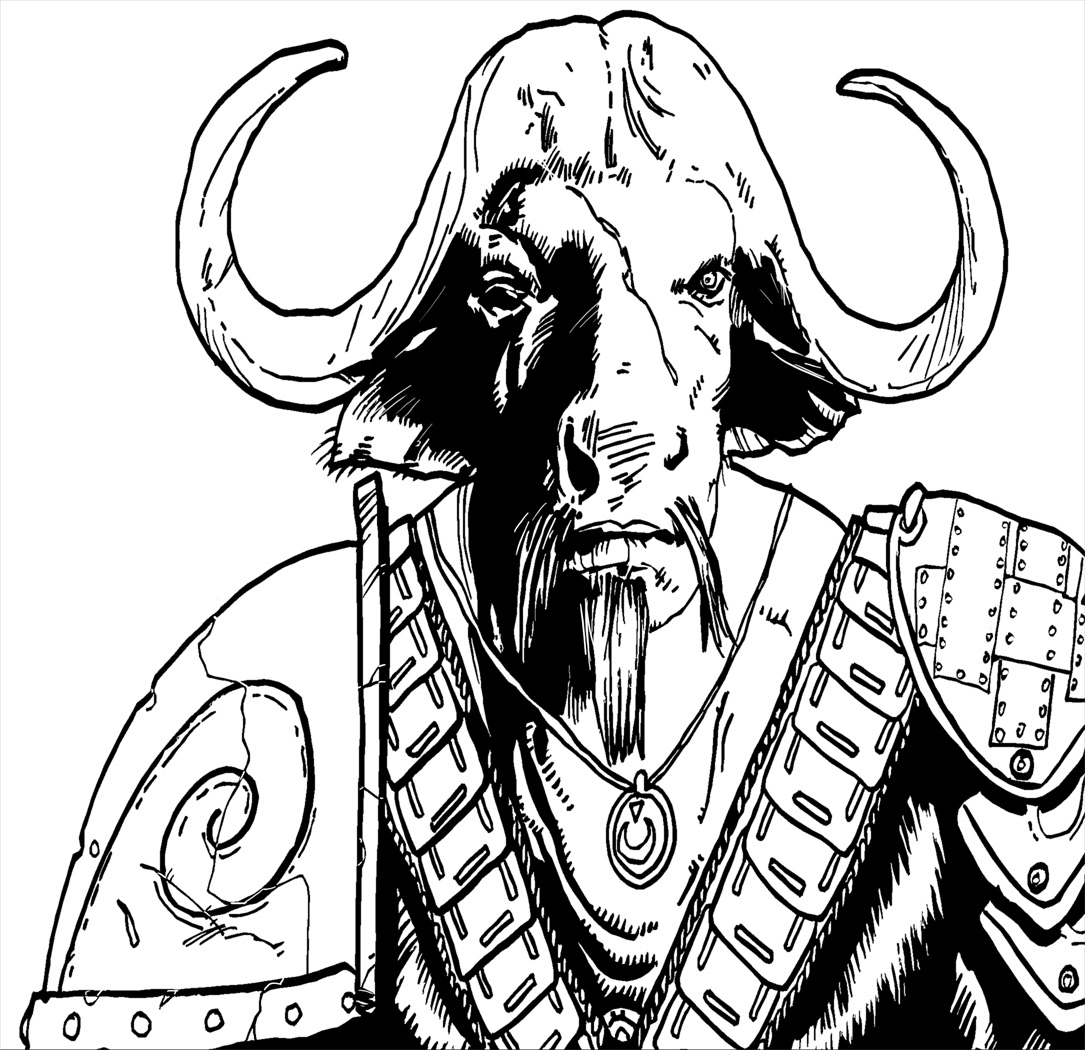
\includegraphics[width=\linewidth]{TCP-Armored-6}

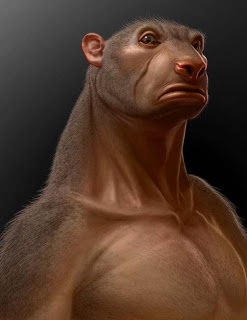
\includegraphics[width=\linewidth]{charlesliu_bearman.jpg}
